\documentclass[12pt,letterpaper,answers]{exam}
%\usepackage{color}
\usepackage[usenames,dvipsnames,svgnames,table]{xcolor}
\usepackage[margin=0.9in]{geometry}
\renewcommand{\familydefault}{\sfdefault}
\usepackage{multicol}
\pagestyle{head}
\definecolor{c02}{HTML}{FFBBBB}
\definecolor{c03}{HTML}{FFDDDD}
\header{AM 111 Problem Set 01 Solution}{}{}
\runningheadrule
\headrule
\usepackage{diagbox}
\usepackage{graphicx} % more modern

\usepackage{amsmath} 
\usepackage{amssymb} 

\usepackage{hyperref}

\usepackage{tcolorbox}
\usepackage[framed,numbered,autolinebreaks,useliterate]{mcode}

\usepackage{nicefrac, listings}

% Set-up for hypertext references
\usepackage{hyperref,color,textcomp,graphicx}
\definecolor{webgreen}{rgb}{0,.35,0}
\definecolor{webbrown}{rgb}{.6,0,0}
\definecolor{RoyalBlue}{rgb}{0,0,0.9}
\hypersetup{
   colorlinks=true, linktocpage=true, pdfstartpage=3, pdfstartview=FitV,
   breaklinks=true, pdfpagemode=UseNone, pageanchor=true, pdfpagemode=UseOutlines,
   plainpages=false, bookmarksnumbered, bookmarksopen=true, bookmarksopenlevel=1,
   hypertexnames=true, pdfhighlight=/O,
   urlcolor=webbrown, linkcolor=RoyalBlue, citecolor=webgreen,
   %pdfauthor={Chris H. Rycroft},
   %pdfsubject={Harvard AM227 (Fall 2019)},
   pdfkeywords={},
   pdfcreator={pdfLaTeX},
   pdfproducer={LaTeX with hyperref}
}

\def\been{\begin{enumerate}}
\def\enen{\end{enumerate}}
\def\beit{\begin{itemize}}
\def\enit{\end{itemize}}
\def\dsst{\displaystyle}
\def\dx{\Delta x}
\hyphenation{}
\newcommand{\blank}[1]{\underline{\hspace{#1}}}

\makeatletter
\def\SetTotalwidth{\advance\linewidth by \@totalleftmargin
\@totalleftmargin=0pt}
\makeatother

\begin{document}
 \pdfpageheight 11in 
  \pdfpagewidth 8.5in

Problem set answers and/or solutions are provided below.  If you would like additional solution steps for any questions, ask for them on Ed or at office hours, and we will provide those.
  
\begin{questions}
\question (binary and floating point)
\begin{parts}
\part (Sauer \S0.2: 1ac, 2ac): Find the binary representation of the base $10$ numbers:
\begin{subparts}
\item $64$
\item $79$
\item $1/8$
\item $35/16$
\end{subparts}

\begin{EnvFullwidth}
\begin{solution}
\begin{subparts}
\item $(1000000)_2$
\item $(1001111)_2$
\item $(0.001)_2$
\item $(10.0011)_2$
\end{subparts}
\end{solution}
\end{EnvFullwidth}

\part (Sauer \S0.3: 2ac): Express the following base $10$ numbers as floating point numbers.  Use the Rounding to Nearest Rule.  

% https://www.tutorialandexample.com/different-kinds-of-boxes-in-latex
Example notation for expressing the floating point number (have 52 bits in the box):
\[\text{fl}(\frac{1}{3}) = +1.\ \framebox[11cm][l]{0101010101010101010101010101010101010101010101010101}\times 2^{-2}\]
\begin{subparts}
\item $9.5$
\item $100.2$
\end{subparts}

\begin{EnvFullwidth}
\begin{solution}
\begin{subparts}
\item $\text{fl}(9.5)=+1.\ \framebox[11cm][l]{0011000000000000000000000000000000000000000000000000}\times2^3$
\item $\text{fl}(100.2)=+1.\ \framebox[11cm][l]{1001000011001100110011001100110011001100110011001101}\times2^6$
\end{subparts}
\end{solution}
\end{EnvFullwidth}

\part (Sauer \S0.3: 9)

Explain why you can determine machine epsilon on a computer using floating point numbers with rounding to nearest by calculating $(7/3 - 4/3) - 1$.

Does $(4/3 - 1/3) - 1$ also give $\epsilon_{\text{mach}}$?

To provide your explanation, convert to floating point numbers and carry out the machine arithmetic.

\SetTotalwidth
\begin{solution}
$(\nicefrac{7}{3})_{10} = 1.00\overline{10}\times2^1$, and after rounding, $\text{fl}\left(\nicefrac{7}{3}\right) = 1.0010...10101011\times2^1$.

$(\nicefrac{4}{3})_{10} = 1.\overline{01}\times2^0$, and after rounding, $\text{fl}\left(\nicefrac{7}{3}\right) = 1.01...01010101\times2^0$. Subtracting gives
\begin{align*}
     & 1.\ \framebox[11cm][l]{0010101010101010101010101010101010101010101010101011}0\times2^1 \\
    -& 0.\ 1\framebox[11cm][l]{0101010101010101010101010101010101010101010101010101}\times2^1 \\
    =& 0.\ 1\framebox[11cm][l]{0000000000000000000000000000000000000000000000000001}\times2^1
\end{align*}
that is normalized to
$$1.\ \framebox[11cm][l]{1000000000000000000000000000000000000000000000000001}\times2^0$$
which is $1+\epsilon_\text{mach}$. After subtracting 1, the result is that the double precision floating point version of $(\nicefrac{7}{3}-\nicefrac{4}{3})-1$ is $\epsilon_\text{mach}$.

$(\nicefrac{4}{3})_{10} = 1.\overline{01}\times2^0$, and after rounding, $\text{fl}\left(\nicefrac{7}{3}\right) = 1.01...01010101\times2^0$.

$(\nicefrac{1}{3})_{10} = 1.\overline{01}\times2^{-2}$, and after rounding, $\text{fl}\left(\nicefrac{1}{3}\right) = 1.01...01010101\times2^{-2}$. Subtracting gives
\begin{align*}
     & 1.\ \framebox[10.9cm][l]{0101010101010101010101010101010101010101010101010101}00\times2^0 \\
     -& 0.\ 01\framebox[11cm][l]{0101010101010101010101010101010101010101010101010101}\times2^0 \\
    =& 0.\ 1\framebox[10.9cm][l]{1111111111111111111111111111111111111111111111111111}1\times2^0
\end{align*}
that is normalized to
$$1.\ \framebox[11cm][l]{1111111111111111111111111111111111111111111111111111}1\times2^{-1}$$
and rounds to
$$1\ \framebox[11cm][l]{0.000000000000000000000000000000000000000000000000000}\times2^{-1}$$
which is $1.0\times2^0$. After subtracting $1$, the result is machine zero, not $\epsilon_\text{mach}$.

(As a fun experiment, try typing \texttt{13/3, 10/3, 7/3, 4/3, 1/3} in Python and see the returned numbers. What do you notice about their last digits? Can you explain the pattern?)

\end{solution}

\end{parts}

\question (condition number) (based on Greenbaum and Chartier \S6.3: 5)

Suppose $a_0$ dollars are deposited in a bank paying $5\%$ interest per year.  When the interest compounds $n$ times per year, the amount in the account after the first compounding will be $a_0\left(1+\dfrac{0.05}{n}\right)$.

At the next compounding, the interest is paid on $a_0\left(1+\dfrac{0.05}{n}\right)$ so the amount will be \[\left(a_0\left(1+\dfrac{0.05}{n}\right)\right)\left(1+\dfrac{0.05}{n}\right) = a_0\left(1+\dfrac{0.05}{n}\right)^2.\]  After one year ($n$ compoundings), the amount will be $a_0\left(1+\dfrac{0.05}{n}\right)^n$.

Let $\mathcal{I}_n(x) = \left(1+\dfrac{x}{n}\right)^n$, the \emph{compound interest formula}.
\begin{parts}
\item Find an expression for the relative condition number, $\kappa_{\mathcal{I}_n}(x)$, for $\mathcal{I}_n(x)$.

For $x = 0.05$ would you consider the problem to be well conditioned?  Ill conditioned?  Does your assessment vary with $n$?  Provide a brief justification/explanation.

\SetTotalwidth
\begin{solution}
Plug in the relative condition number formula, we have
$$\kappa_{\mathcal{I}_n}(x) = \left\lVert x \frac{(1+\frac{x}{n})^{n-1}}{(1+\frac{x}{n})^n} \right\rVert = \left\lVert \frac{x}{1+\frac{x}{n}} \right\rVert$$
When $x=0.05$, the follow inequality holds (it is always true for any $x, n>0$ because $1+\nicefrac{x}{n}>1$):
$$\kappa_{\mathcal{I}_n}(x)<\lVert x \rVert \quad\Longrightarrow\quad \kappa_{\mathcal{I}_n}(x)\bigg|_{x=0.05}<0.05$$
In terms of well-conditioned or ill-conditioned, please check the \href{https://edstem.org/us/courses/24695/discussion/1746969?answer=3974365}{Ed Discussion post}. For $\kappa_{\mathcal{I}_n}(x)$, it will be much smaller than $0.05$ for small $n$, but it will converge to $0.05$ for big $n$. Your work is considered ``Correct" (or ``Satisfactory") so long as you provide a valid justification/explanation.
\end{solution}

\item For fixed $x$, $\lim\limits_{n\rightarrow\infty}\mathcal{I}_n(x) = e^x$

Use the Python code below to see values of $\mathcal{I}_n(x)$ for $n=1,10,100,1000,...,10^{19}$.

(type this code in or find it on Canvas/github/FAS On Demand)

\begin{verbatim}
n = 1
x = 0.05
interest_of_x = []
for val in range(0, 20):
    interest_of_x.append(['{:.3e}'.format(n), (1+x/n)**n])
    n = 10*n
# print formatting help from
# https://stackoverflow.com/questions/58722579/python-print-list-of-numbers-in-scientific-notation#58722625

print(*interest_of_x, sep='\n')
# more print formatting help from
# https://www.geeksforgeeks.org/print-lists-in-python-4-different-ways/
\end{verbatim}
\vspace{0.1in}

Compare these values to
\begin{verbatim}
import numpy as np

np.exp(x)
\end{verbatim}

For which $n$ are $\mathcal{I}_n(x)$ and $e^x$ closest?

Does your calculation converge to $e^x$ as $n$ increases?

\SetTotalwidth
\begin{solution}
When $n=10^7$, $\mathcal{I}_n(x)$ and $e^x$ are the closest. No, it does not converge.
\end{solution}

\item For the value of $n$ you chose as yielding the closest value to $e^x$, treat $\left(1+\dfrac{x}{n}\right)^n$ as an approximation to $e^x$.  

For this $n$, compute the condition number from your values: 

$x = 0.05$, 

$y = e^x$, 

$\hat{y} = \left(1+\dfrac{x}{n}\right)^n$, 

and $e^{\hat{x}}=\hat{y}$.  

Compare this to your condition number from part (a).
 
\SetTotalwidth
\begin{solution}
When $n=10^7$, the condition number from part (a) is
$$\kappa_\text{part(a)}= \left\lVert \frac{0.05}{1+\frac{0.05}{10^7}} \right\rVert = 0.04999999975$$
For the computed condition number, we need to first find $\hat{x}$ then apply the formula:
\begin{lstlisting}[language=Python]
import numpy as np
    
n = 10**7
x = 0.05
y = np.exp(x)

y_hat = (1.0 + x/n)**n
x_hat = np.log(y_hat)

k_x = (x - x_hat) / x
k_y = (y - y_hat) / y
kappa = k_y / k_x

print(kappa)
\end{lstlisting}
You would find \texttt{kappa = 0.05000000796325147}. The two condition numbers are close but not the same. In particularly, the computed \texttt{kappa} should be less than $0.05$. But due to the accumulative machine precision errors per-multiplication, it actually becomes larger than $0.05$.
\end{solution}

For $n = 10^{18}$ or $n = 10^{19}$, what happens to the calculation in part (b)?  Can this error be explained by the condition number?  If not, provide an alternate explanation.

\SetTotalwidth
\begin{solution}
When $n = 10^{18}$ or $n = 10^{19}$, the calculation in part (b) gives poor estimation (i.e. goes to $1$). This error is not due to the condition number but machine precision. In Python, the machine precision of the floating point number system is at the order of magnitude of $10^{-16}$. Therefore, any number that is smaller than this value will not be represented. In part (b), we are repeatedly adding a small number \texttt{x/n} to $1$. When $n = 10^{18}$ or $n = 10^{19}$, this number is at the order of magnitude of $10^{-21}$ and $10^{-22}$, i.e. considered as $0$ in Python. In conclusion, in the Python floating point number system, we have
$$\left(1+\frac{x}{n}\right)^n \approx \left(1+0\right)^n = 1 \quad\forall\quad n>14, n\in\mathbb{N}$$
\end{solution}

\end{parts}

\question (more floating point) (from Ciocanel Spring 2022)
\begin{parts}
\item 
 Write a program to determine the machine error of either a \texttt{float16}, \texttt{float32}, or \texttt{float64} in Python.

To do this, \texttt{import numpy as np} and set \texttt{epsilon = np.float64(1.0)}.  (Use \texttt{float16} or \texttt{float32} for all math if you prefer).

Create a loop, and each time through the loop assign \texttt{x = np.float64(1.0) + epsilon}.  Then divide \texttt{epsilon} by $2$ (\texttt{epsilon = epsilon/np.float64(2)}).

Continue looping until the value of  \texttt{np.float64(1.0)+epsilon} is no longer greater than $1$.

\emph{You might use a \texttt{while} loop for this}.

Use your results to determine the number of bits in the mantissa of the data type.

\emph{Each division by $2$ is shifting the decimal/binary/radix point of your binary number, so counting these divisions could help.  \texttt{np.log2} could also help.}

\SetTotalwidth
\begin{solution}
For ``Correct", you need to report both the machine error and the number of bits in the mantissa. You should include a counter in your while-loop to count the mantissa bits. Below is an example code (assuming \texttt{numpy} has been imported):
\begin{lstlisting}[language=Python]
epsilon = np.float64(1.0)
counter=0

while np.float64(1.0) + epsilon > 1:
    x = np.float64(1.0) + epsilon
    epsilon /= np.float64(2.0)
    counter += 1

print(epsilon, counter)
\end{lstlisting}
You would have \texttt{epsilon = 1.1102230246251565e-16, counter = 53} for \texttt{float64}. (Technically the mantissa for \texttt{np.float64} has \href{https://en.wikipedia.org/wiki/Double-precision_floating-point_format}{52 bits} explicitly stored.)
\end{solution}

\part Write a program to determine the overflow of a float of your choice.

 Initialize a variable \texttt{r = np.float32(1.0)} (or \texttt{float16} or \texttt{float32}).
 
 Create a loop that prints out a value for \texttt{r = np.float32(1.0)} and for \texttt{np.log2(r)} and then doubles \texttt{r} each time through the loop (be sure \texttt{r} remains the correct type of float when you double it).  Repeat until the value of \texttt{r} becomes infinite.  Find the value \texttt{k}, where \texttt{r = 2**k} for the largest \texttt{r} before overflow.

\SetTotalwidth
\begin{solution}
For ``Correct", you need to have a loop that prints out \texttt{r} and \texttt{np.log2(r)}, and report the value \texttt{k}. You should include a counter in your loop to find \texttt{k}. Below is an example code (assuming \texttt{numpy} has been imported):
\begin{lstlisting}[language=Python]
r = np.float16(1.0)
k = 0

while r != np.infty:
    k += 1
    r = r * np.float16(2.0)
    print("r:", r, "log2(r):", np.log2(r))

print("k:", k)
\end{lstlisting}
You would have \texttt{k = 16} for \texttt{float16}.
\end{solution}
 
\item To check your work, compare your results to information about the data type in Python.  You can find that info using following commands

\begin{verbatim}
print(np.finfo(np.float16()))
print(np.finfo(np.float32()))
print(np.finfo(np.float64()))    
\end{verbatim}


\end{parts}

\question (Calculus review) (Sauer \S0.5) Review the Fundamentals of Calculus section in Sauer 2017. 

\emph{Find a copy on Canvas.} 
\begin{parts}
\item Complete Sauer \S0.5: 3ab
\item Complete Sauer \S0.5: 5ab
\end{parts}

\SetTotalwidth
\begin{solution}
Answers are here.  Ask for solution steps if desired.
\begin{parts}
\item
    \begin{subparts}
    \item $c=\nicefrac{2}{3}$
    \item $c=\nicefrac{1}{\sqrt{2}}$
    \end{subparts}
\item
    \begin{subparts}
    \item $1 + x^2 + \frac{1}{2}x^4$
    \item $1 - 2x^2 + \frac{2}{3}x^4$
    \end{subparts}
\end{parts}
\end{solution}


\question (Numerical error in a stock index) \emph{(Thomas Fai, AM 111 Spring 2017.  See example in Greenbaum and Chartier) }

\textbf{Read this problem in its entirety before beginning work on it.}


A famous example of roundoff error was a short-lived index devised at the Vancouver stock exchange\cite{quinn1983}. The index contained 1400 stocks listed on the exchange, and each stock was weighted equally in determining the value of the index (most other indexes are weighted so that large companies count more than small ones). At the time the index was started in January 1982, the sum of the initial selling prices of all 1400 stocks (the baseline sum) was rescaled to give the index an initial value of 1000.

Taken together, the stocks in this index underwent changes in price a total of 2800 times per day. Each time one of the stocks changed its price, the index was updated as follows:

\[\text{New Index} = \text{Old Index} + (\text{Change in Stock Price})\dfrac{1000}{\text{Baseline Sum}}\]

Then, after each change, the index was truncated after the third decimal place. For example, if after a change in stock price the index stood at 735.32567, the computer simply dropped the last two digits, making it 735.325.
\begin{parts}
\part Write two functions:
\begin{itemize}
\itemsep0pt
    \item function \texttt{truncate(x)} that returns \texttt{trunc\_x}, a truncation of the number $x$ after the third decimal place.
    
    
% \href{https://numpy.org/doc/stable/reference/generated/numpy.floor.html}{Link: You may choose to use the floor function in numpy - there are other ways to do this as well}

    \item function \texttt{update\_index(old\_index, delta, baseline\_sum)} that returns \texttt{new\_index}, as defined above.  \texttt{delta} is the change in stock price of a single stock, \texttt{old\_index} is the previous value of the index, and \texttt{baseline\_sum} is the original sum of the stock prices
\end{itemize}

Find commenting conventions for Python \href{https://peps.python.org/pep-0257/}{here}.

\begin{solution}
\begin{verbatim}
import numpy as np
def truncate(x):
    # truncate after three decimal places
    return np.floor(x*1000)/1000

truncate(1.23456)

def update_index(old_index, delta, baseline_sum):
    return old_index + delta*1000/baseline_sum
\end{verbatim}
\end{solution}

\part Write a program that simulates the evolution of this index over time.

\begin{solution}
\begin{verbatim}
# random number code from https://datagy.io/python-random-number/
# Generate a list of random integers and convert to dollars + cents 
#  (divide by 100)
import random

random_list = [random.randint(0, 20000)/100 for j in range(1400)]
# print(random_list)

baseline_sum = truncate(np.sum(random_list))
index_value = []
total_daily_delta = []
old = 1000
for j in range(20*22):
    list_of_deltas = [random.randint(-200, 200)/100 for j in range(2800)]
    for delta in list_of_deltas:
        new = truncate(update_index(old,delta,baseline_sum))
        index_value.append(new)
        old = new
    total_daily_delta.append(sum(list_of_deltas))
\end{verbatim}
\end{solution}

%\emph{Submit a pdf on Gradescope.}

\part List any assumptions you made about how the market works as part of your simulation.

\begin{solution}
\begin{enumerate}
\itemsep0pt
    \item $1400$ stocks
    \item $2800$ trades on each trading day
    \item each trade is for a number between $-2$ to $2$ dollars (in dollars and cents)
    \item the initial stock values range from $0$ to $200.00$ dollars.
    \item assume there are $20$ trading days in a month so $20*22$ trading days in $22$ months
\end{enumerate}
\end{solution}

\part Plot the evolution of the index over the first day, and over a $22$ month period (you can assume all months have the same number of trading days).

 Write a brief description of what you see in your plot.
 
 \begin{solution}
 \begin{verbatim}
import matplotlib.pyplot as plt
# one day
time_vals = np.linspace(0,1,2800)
plt.plot(time_vals,index_value[0:2800])
plt.ylim([997, 1001])
plt.xlabel('time (days)')
plt.ylabel('index value')
plt.show()
# 22 months
time_vals = np.linspace(0,22,2800*20*22)
plt.plot(time_vals,index_value)
plt.xlabel('time (months)')
plt.ylabel('index value')
 \end{verbatim}
 
 Plot the first day of the simulation, so the first $2800$ trades.
 
 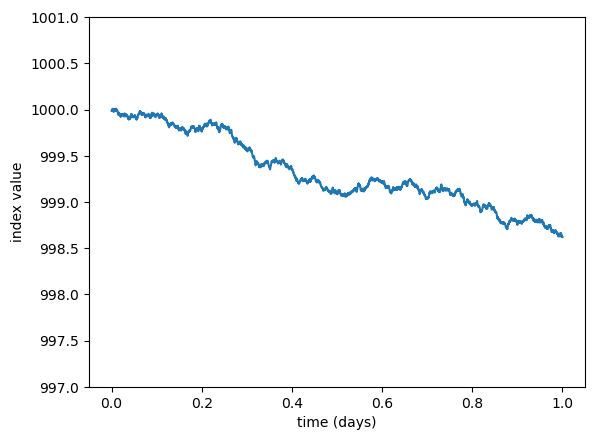
\includegraphics[width=0.7\textwidth]{img/PSet02onedaystock.png}

 
 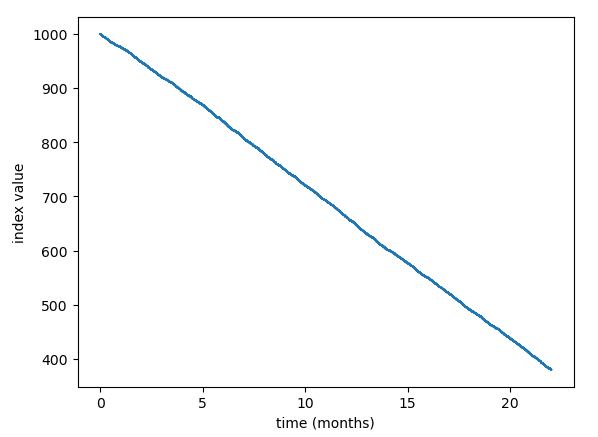
\includegraphics[width=0.7\textwidth]{img/PSet02stock22months.png}
 
  The index is declining (on average) over the course of the day and over the course of 22 months.
 
 \end{solution}

\item Given the truncation procedure used in updating the index, by how many points, on average, would you expect the index to drop from one change of stock price?  What about in 1 day? Or in 22 months?

\begin{solution}
On average $0.0005$ is truncated on every update of the index, so a loss of $2800*0.005 = 1.4$ over a day and a loss of $20*22*1.4 = 616$ over $22$ months of trading days.
\end{solution}

\item After 22 months, the actual index stood at 524.881. What can you infer about the evolution of the market during this time: was it a bull market or a bear market? Explain your thinking.

\begin{solution}
The average loss would be $616$ leaving the index below $400$ so for it to be at $524$ the market would need to be good (bull).
\end{solution}

\item Make a suggestion for how to modify the procedure used to update the index. Implement your modification (you will need to write a new function to replace the function truncate from part (a)). Plot the evolution of your modified index over 1 day and over 22 months.  Compare your modified index to the evolution of the actual index (compare the indices using identical values of the change in stock price at all time points). What do you observe?

\begin{solution}
Replace truncation with rounding.  This appears to fix the index.
\end{solution}

\item If you have spent more than 9 hours on this problem set, write a note to that effect and skip this problem or parts of this problem.  

\end{parts}


This problem is provided without information about the Python functions you might use to complete it, and without guidance for some of the assumptions you'll need to make about the index.  

If you'd like more information/guidance, ask us on the Ed discussion board


\end{questions}



\bibliographystyle{plain}
\bibliography{references.bib}
\end{document}
